\documentclass[letterpaper,12pt]{article}
\usepackage{fancyhdr}
\usepackage{amsfonts,amsmath,amsthm,amssymb,mathtools,empheq,array}
\usepackage{pgfplots,float,parskip,nameref,graphicx,subfig}
\usepackage[font=small,labelfont=bf]{caption}
\usepackage{pythonhighlight}

\renewcommand{\thefootnote}{\fnsymbol{footnote}}

\graphicspath{{../../.used/figures/}{../assets/}}
\pagestyle{fancy}
\fancyhf{}
\lhead{Fall 2023}
\rhead{Writeup 1}
\rfoot{\thepage}
\title{Computationally Modeling Propagation of a Wave Packet}
\author{Seth Eshraghi}
\date{\today}

\begin{document}

    \maketitle
    \thispagestyle{empty}

    \begin{abstract}
        To calculate expected values of physical observables such as dipole
        moment, velocity, and acceleration, I represented a wave packet with a
        Gaussian envelope as a column vector in discrete space and solved a
        linear systems problem to compute propagations at different time steps
        using the implicit propagation scheme. The wave packet is in a box,
        whose size emulates infinte space. Certain consequences of discretizing
        space and time are assessed. Using different parameters, particularly
        the center wave number and width of a potential well, I discovered that
        computational calculations for transmission in a system with a finite
        square potential well might align with the analytically derived
        transmission coefficient.
    \end{abstract}

    \newpage

    \pagenumbering{roman}
    \tableofcontents
    \listoffigures

    \newpage

    \pagenumbering{arabic}
    \addcontentsline{toc}{section}{Introduction}
\section*{Introduction}

Computationally studying a physical observable of a single-electron atom may
require the use of a wave function represented in a computer.  To compute
the expected value of any physical quantity, one may make use of the
probability distribution function (PDF) definition of expected value. The
square magnitude of a solution to the Schrödoinger equation over position at
a given time may be used as a PDF if it is normalized. It is very difficult
to determine the state of a wave function at a given time in some systems by
analytical methods, so computational modeling of the wave functions is used.

I used the implicit scheme given an initial discretized wave function to
propagate the wave function through discrete time. The implicit scheme and
discretization of time and space introduces some limitations, but these
limitations are predictable. This will allow for easier computation of
expected values for physical quantities of interest, such as dipole
acceleration, on an atomic level, which can be rescoped to a macro-level
system using Maxwell's equations. This process can aid in understanding and
manipulating certain atomic and molecular processes when combined with
experimental methods such as utilizing high harmonic generation to create
attosecond pulses of light.

The programs implement a basic particle-in-a-box system. The wave packet was
constructed by multiplying a Gaussian function by a plane wave equation, and
its evolution was computed iteratively by the implicit scheme of
propagation. We investigate a system with constant potential energy as well
as a potential well. The programs are verified by comparing computationally
calculated expected values to those which were analytically calculated as
well as assessing the autocorrelation. The results of different condidtions
are examined graphically, and physical and mathematical explanations to
those results are provided.


    \newpage

    \addcontentsline{toc}{section}{Theory}
\section*{Theory}

Storage and memory on computers are finite, so a wave function or packet and
the dynamics of it must be represented discretely. Both time and space are
discretized into a grid with units $\delta t$ and $\delta x$, respectively,
and we work within one dimension of space. We choose units such that $\hbar$
is equal to one, and we assume that mass is one. Unless stated otherwise,
change is assumed to be with respect to time.

\addcontentsline{toc}{subsection}{Implicit Scheme of Propegation}
\subsection*{Implicit Scheme of Propagation}

I chose to implicitly propegate a wave function by virtue of computational
simplicity. We start with the time-dependent Schrödinger equation.

\[
    \hat{H} \Psi(x, t) = \hat{E} \Psi(x, t)
\]

where $\hat{H} = \frac{\hat{p} ^ 2}{2} + V(x)$. We may express the energy
operator explicitly and then solve differential equation for $\Psi$.

\begin{align*}
    \hat{H} \Psi(t)
    &= i\frac{\partial}{\partial t} \Psi(t) \\
    \frac{\partial}{\partial t} \Psi(t)
    &= -i\hat{H} \Psi(t) \\
    \Psi(t) &= e^{-i\hat{H} t} \Psi(0) \\
    \Psi(t) &=
    \frac{e^{-i\hat{H} \frac{t}{2}}}{e^{i\hat{H} \frac{t}{2}}} \Psi(0)
\end{align*}

We expand both the numerator and the denomenator of the operator into a
first degree Maclaurin series.

\[
    \left( 1 + i\hat{H} \frac{t}{2} \right) \Psi(t) \approx
    \left( 1 - i\hat{H} \frac{t}{2} \right) \Psi(0)
\]

\pagebreak

Considering that we are working in discrete space and time, we have

\begin{equation}
    \left( 1 + iH \frac{\delta t}{2} \right) \vec{\Psi}(\delta t) \approx
    \left( 1 - iH \frac{\delta t}{2} \right) \vec{\Psi}(0)
    \label{eq:impsch}
\end{equation}

where $H$ is the matrix representation of the Hamiltonian operator and
$\vec{\Psi}(t)$ is the column vector representation of $\Psi(t)$ such that
$\vec{\Psi}(t)_j$ is the value of $\Psi(t)$ at $x = j \cdot \delta x$. The
wave function at the next time step is computed by solving the linear system
through forward elimination and backsubstitution.

\paragraph{Total Energy} Suppose we have a wave fuction representing a plane
wave, $\psi(x) = e^{ikx}$. Assuming $\hat{H} = \frac{\hat{p}^2}{2}$, we have,
in discrete space, from the time-independent Schödinger equation

\[
    -\frac{1}{2}\vec{\psi}_x'' = E \vec{\psi}_x.
\]

Now we take the numerical second derivative of $\vec{\psi}_x$ by calculating
the sum of the Taylor series expansions for $\vec{\psi}_{x - \delta t}$ and
$\vec{\psi}_{x + \delta t}$ and then solve for $E$.

\begin{gather*}
    -\frac{\vec{\psi}_{x - \delta t} - 2\vec{\psi}_x + \vec{\psi}_{x +
    \delta t}}{2 \delta t^2} + \mathcal{O}\left[\delta t^2\right]
    = E \vec{\psi}_x
    \\
    -e^{ikx}
    \left(
    \frac{e^{-ik\delta t} + e^{ik\delta t} - 2}{2 \delta t^2}
    \right)
    \approx E e^{ikx}
    \\
    -\frac{2\cos(k)\delta t - 2}{2\delta t^2} \approx E
\end{gather*}

\pagebreak

We examine the behavior of energy as the time step becomes small.

\begin{align}
    \lim_{\delta t \to 0} E
    &\approx
    \lim_{\delta t \to 0} -\frac{\cos{k\delta t} - 1}{\delta t^2}
    \nonumber
    \\
    &\approx \lim_{\delta t \to 0} \frac{k\sin{k\delta t}}{2\delta t}
    \nonumber
    \\
    &\approx \lim_{\delta t \to 0} \frac{k^2\cos{k\delta t}}{2}
    \nonumber
    \\
    &\approx \lim_{\delta t \to 0}
    \frac{k^2 \left( 1 - \frac{(k\delta t) ^ 2}{2} \right) +
    \mathcal{O}\left[\delta t^4\right]}{2}
    \nonumber
    \\
    E &\approx \frac{k^2}{2}
    \label{eq:EnoV}
\end{align}

Note that the energy in discrete space varies with the time step and will
never be exactly $\frac{k^2}{2}$ as stored in the computer. Additionally,
the maximum energy of the wave is given by $\frac{2}{\delta x^2}$.

\paragraph{Error} In our derivation of equation \eqref{eq:impsch}, we
approximated the exponential operators by truncating the Taylor series
expansions of them. Note that $e^{-i\hat{H}t} \approx
\frac{1 - iH\frac{\delta t}{2}}{1 + iH\frac{\delta t}{2}}$. If we expand the
left side of the approximate equation to its Maclaurin series and multiply
both sides by $1 + iH\frac{\delta t}{2}$, then we arrive at

\[
    1 - i\hat{H}\frac{\delta t}{2} - i\hat{H}^3\frac{\delta t^3}{12}
    \approx
    1 - iH\frac{\delta t}{2}
\]

so the error for the propagation operator is on the order of $\hat{H}^3
\delta t^3$. This error will propagate through time.

\paragraph{Unitary Operator} Because of the numerical second derivative, we
know that $H$ is a tridiagonal real matrix, so it is Hermitian as an
operator. In order to use the wave function to calculate expected values,
the square magnitude of the wave function must be a PDF over $x$.
Therefore, the wave function's square magnitude integrated over all $x$ (or
in discrete space, the norm) must equal to one for all time, so our operator
in equation \eqref{eq:impsch} should be unitary.

\begin{align*}
    \left(
    \frac{1 - iH\frac{\delta t}{2}}{1 + iH\frac{\delta t}{2}}
    \right)^\dag
    \left(
    \frac{1 - iH\frac{\delta t}{2}}{1 + iH\frac{\delta t}{2}}
    \right)
    &=
    \frac{\left(1 + iH^\dag\frac{\delta t}{2}\right)
    \left(1 - iH\frac{\delta t}{2}\right)}
    {\left(1 - iH^\dag\frac{\delta t}{2}\right)
    \left(1 + iH\frac{\delta t}{2}\right)}
    \\
    &=
    \frac{\left(1 + iH\frac{\delta t}{2}\right)
    \left(1 - iH\frac{\delta t}{2}\right)}
    {\left(1 - iH\frac{\delta t}{2}\right)
    \left(1 + iH\frac{\delta t}{2}\right)}
    \\
    &= 1
\end{align*}
\vspace{-0.9cm}

\addcontentsline{toc}{subsection}{Model Boundary Conditions and Parameters}
\subsection*{Model Boundary Conditions and Parameters}
We model a one-dimensional particle in a box, where the wave packet is in an
infinite potential well bounded at $x = 0, R$, where $R$ is large enough to
emulate an infinite $x$ space for the wave packet. As the potential energy
tends toward infinity, we see that the magnitude of the wave function is
equal to 0 at at the $x$ boundaries. To reiterate, the grid spacing for time
and space is given by $\delta t$ and $\delta x$ respectively. Finally, we
propagate for a definite time. Also note the the parameters for a Gaussian
wave packet such as the wave number and standard deviation.

\addcontentsline{toc}{subsection}{Computer Representation of the Hamiltonian
and Wave Function}
\subsection*{Computer Representation of the Hamiltonian and Wave Function}

\paragraph{Wave Function as a Column Vector}
A wave packet is a superposition of plane waves that have a nonzero range
in wave number and angular frequency which forms a Gaussian envelope. For a
given time, it can be created by the form

\vspace{-0.5cm}
\[
    \Psi(x) = G(x)e^{ikx}
\]

where $\Psi$ is a wave packet, $G$ a gaussian function, and $e^{ikx}$ a
plane wave expression. For storing on a machine, I represented $\Psi(x)$ as

\vspace{-0.2cm}
\[
    \vec{\Psi}(t) =
    \begin{bmatrix}
        \Psi(1 \delta x, t) \\
        \Psi(2 \delta x, t) \\
        \vdots \\
        \Psi(N \delta x, t) \\
    \end{bmatrix}
    =
    \begin{bmatrix}
        \Psi_1(t) \\
        \Psi_2(t) \\
        \vdots \\
        \Psi_N(t) \\
    \end{bmatrix}
\]

where $N$ is the number of grid spaces on $x$.

\paragraph{The Propagator Matrix}

Let us denote $V(j \delta x)$ as $V_j$. Equation \eqref{eq:impsch} can be
expanded to

\begin{gather}
    \scalebox{0.7}{$
    \Psi_j(\delta t) + i\frac{\delta t}{2}
    \left(
    -\frac{\Psi_{j-1}(\delta t)-2\Psi_j(\delta t)+\Psi_{j+1}(\delta t)}
    {2 \delta x^2}
    + V_j \Psi_j(\delta t)
    \right)
    $}
    =
    \scalebox{0.7}{$
    \Psi_j(0) - i\frac{\delta t}{2}
    \left(
    -\frac{\Psi_{j-1}(0)-2\Psi_j(0)+\Psi_{j+1}(0)}
    {2 \delta x^2}
    + V_j \Psi_j(0)
    \right)
    $}
    \nonumber
    \\
    \scalebox{0.65}{$
    \begin{bmatrix}
        1 + i\frac{\delta t}{2}\left(V_1 + \frac{1}{\delta t^2}\right)
        &
        -i\frac{\delta t}{(2 \delta x)^2} & 0 & 0 & 0 & \cdots & 0 \\
        -i\frac{\delta t}{(2 \delta x)^2}
        &
        1 + i\frac{\delta t}{2}\left(V_2 + \frac{1}{\delta t^2}\right)
        & -i\frac{\delta t}{(2 \delta x)^2} & 0 & 0 & \cdots & 0 \\
        0 & \ddots & \ddots & \ddots & 0 & \cdots & 0 \\
        \vdots & & & & & & \vdots \\
        0 & \cdots & \cdots & 0 &
        -i\frac{\delta t}{(2 \delta x)^2}
        &
        1 + i\frac{\delta t}{2}\left(V_2 + \frac{1}{\delta t^2}\right)
        & -i\frac{\delta t}{(2 \delta x)^2}
    \end{bmatrix}
    \begin{bmatrix}
        \Psi_1(\delta t) \\
        \Psi_2(\delta t) \\
        \vdots \\
        \\
        \Psi_N(\delta t)
    \end{bmatrix}
    =
    \vec{\phi}_j(0)
    $}
    \label{eq:prop}
\end{gather}

where the matrix in equation \eqref{eq:prop} is the propagator matrix.

\addcontentsline{toc}{subsection}{Finite Square Potential Well}
\subsection*{Finite Square Potential Well}
A potential well is a region where the wave packet experiences a lower
amount of potential energy. A well can be modeled by defining the potential
energy function $V(x)$ to include a region with a lower value.

In computer implementation, the well must be continuous due to the Gibbs
phenomenon. A smooth square well that does not allow for the occurance of
Gibbs phenomenon can be achieved by using a higher power Gaussian function.
In my modeling, I set the width of the well to be smaller than the width of
the wave packet, which will be discussed in more detail within the
\nameref{sec:Results} section.

\addcontentsline{toc}{subsubsection}{Transmission Coefficient}
\subsubsection*{Transmission Coefficient}
As the wave propagates through the finite potential well, some of it is
reflected backward, and some of it is transmitted through to the other side
of the well.

Suppose a potential well has a width of $2a$ and is centered at $x = 0$,
where the potential $V(x)$ is equal to $-V_0$ for $-a \leq x \leq a$ and $0$
for $x > a$ and $x < -a$. We label the region corresponding to $x < -a$ as
region I, to $-a < x < a$ as region II, to $x > a$ as region III. During our
meetings we solved for the one-dimentional time-independent Schrödinger
equation for when $E > V(x)$ and $E < V(x)$, obtaining

\begin{align*}
    \Psi_\mathrm{I}(x) &= Ae^{ikx} + Be^{-ikx} \\
    \Psi_{\mathrm{II}}(x) &= C\sin(lx) + D\cos(lx) \\
    \Psi_{\mathrm{III}}(x) &= Fe^{ikx}
\end{align*}

where $l = \sqrt{2(E + V_0)}$, $k = \sqrt{2E}$, and the subscript of the
denotation of each function indicates over which region the function is
defined. The requirements to stitch the three functions into one function
which is defined for all $x$ follows the properties of a valid solution to
the Schrödinger equation:

We compute the transmission coefficient ($T$) by definition ($T^{-1} =
\frac{\left| A \right| ^{2}}{\left| F \right| ^{2}}$), substituting $F$ with
equivalent expression in terms of the energy of the wave ($E$) and the depth
of the potential well.

The requirements to stitch the three wave functions into one follows the
properties of a valid solution to the Schrödinger equation:

\begin{gather}
    Ae^{-ika} + Be^{ika} = -C\sin(la) + D\cos(la) \label{eq:stitch1} \\
    C\sin(la) + D\cos(la) = Fe^{ika} \label{eq:stitch2} \\
    ik(Ae^{-ika} - Be^{ika}) = l(C\cos(la) + D\sin(la)) \label{eq:stitch3} \\
    l(C\cos(la) - D\sin(la)) = ikFe^{ika} \label{eq:stitch4}
\end{gather}

Now we solve for $F$ in terms of $l$, $k$, $a$, and $A$. From equation
\eqref{eq:stitch2}, we solve

\begin{equation}
    C = \frac{Fe^{ika} - D\cos(la)}{\sin(la)} \label{eq:CinD}
\end{equation}

and substitute into equation \eqref{eq:stitch4} to solve for

\begin{gather*}
    Fe^{ika}
    \left(
    \frac{ik}{l}\sin(la) - \cos(la)) = -D(\cos^2(la) + \sin^2(la)
    \right)
    \\
    D = Fe^{ika}
    \left(
    \cos(la) - \frac{ik}{l}\sin(la)
    \right)
\end{gather*}

Then we substitute $D$ in terms of $F$ into equation \eqref{eq:CinD} and
simplify. Note $1 - \cos^2(la) = 1 - \frac{1}{2}(1 + \cos(2la)) = 1 -
\frac{1}{2}(1 + 1 - 2\sin^2(la)) = \sin^2(la)$.

\[
    \scalebox{1}{$
    C
    = \frac{Fe^{ika}(1 - \cos^2(la) +
    \frac{ik}{l}\cos(la)\sin(la))}{\sin(la)}
    = Fe^{ika}
    \left(
    \frac{1 - \cos^2(la)}{\sin(la)} + \frac{ik}{l}\cos(la)
    \right)
    $}
\]

\[
    C = Fe^{ika}
    \left(
    \sin(la) + \frac{ik}{l}\cos(la)
    \right)
\]

Note $\cos^2(la) - \sin^2(la) = \cos(2la)$ and $2\cos(la)\sin(la) =
\sin(2la)$. Substituting $D$ and $C$ in terms of $F$ into equation
\eqref{eq:stitch1}, we get

\begin{gather}
    \scalebox{0.9}{$
    Ae^{-ika}
    = Fe^{ika}
    \left(
    -\sin^2(la) - \frac{ik}{l}\cos(la)\sin(la) + \cos^2(la)
    - \frac{ik}{l}\sin(la)\cos(la)
    \right)
    - Be^{ika}
    \nonumber
    $}
    \\
    = Fe^{ika}
    \left(
    \cos(2la) - \frac{ik}{l}\sin(2la)
    \right)
    - Be^{ika}. \label{eq:AinFB}
\end{gather}

Now we substitute this result and $D$ and $C$ in terms of $F$ into equation
\eqref{eq:stitch3} and solve for $B$.

\begin{align*}
    \scalebox{0.8}{$
    Fe^{ika}
    \left(
    -\frac{ik}{l}\sin(2la) + \cos(2la)
    \right)
    - 2Be^{ika}
    $}
    &=
    \scalebox{0.8}{$
    \frac{l}{ik}Fe^{ika}
    \left(
    2\cos(la)\sin(la) + \frac{ik}{l}\cos^2(la) - \frac{ik}{l}\sin^2(la)
    \right)
    $}
    \\
    -2B &= F\sin(2la)
    \left(
    \frac{l}{ik} + \frac{ik}{l}
    \right)
    \\
    B &= i\frac{\sin(2la)}{2kl}(l^2 - k^2)F
\end{align*}

To solve for $F$ in terms of $A$ we substitute $B$, $C$, and $D$ into
equation \eqref{eq:AinFB}.

\begin{gather*}
    Ae^{-ika}
    = Fe^{ika}
    \left(
    \cos(2la) - \frac{ik}{l}\sin(2la)
    - i\frac{\sin(2la)}{2kl}(l^2 - k^2)
    \right)
    \\
    Ae^{-2ika}
    = Fe^{ika}
    \left(
    \cos(2la) -
    \left(
    \frac{ik}{l} + \frac{i(l^2 - k^2)}{2lk}
    \right)
    \sin(2la)
    \right)
    \\
    F = \frac{e^{-2ika}A}{\cos(2la) - i
    \left(
    \frac{k^2 + l^2}{2kl}
    \right)
    \sin(2la)}
\end{gather*}

Finally, we compute $T^{-1}$ and rewrite it in terms of $E$ and $V_0$.

\begin{gather*}
    T^{-1} = \frac{\left| A \right| ^{2}}{\left| F \right| ^{2}}
    = \frac{\left| A \right| ^{2}}{
        \frac{\left| e^{-2ika} \right| ^2 \left| A \right | ^2}{
                \left|
                \cos^2(2la) + i \left( \frac{k^2 + l^2}{2kl} \right)
                \sin(2la)
                \right| ^2
            }
        }
    = \cos^2(2la) + \left( \frac{(k^2 + l^2)^2}{4k^2l^2} \right) \sin^2(2la)
    \\
    = 1 - \sin^2(2la) + \left( \frac{(k^2 + l^2)^2}{4k^2l^2}
    \right) \sin^2(2la)
    = 1 + \left( \frac{k^4 - 2k^2l^2 + l^4}{4k^2l^2} \right) \sin^2(2la)
    \\
    = 1 + \left( \frac{4E^2 - 8E(E + V_0) + 4(E^2 + 2EV_0 + V_0^2)}
    {16E(E + V_0)} \right) \sin^2(2a\sqrt{2(E + V_0)}
\end{gather*}

\begin{center}
    \boxed{
        T = \frac{1}{1 + \left( \frac{V_0}{4E(E + V_0)} \right)
        \sin^2(2a\sqrt{2(E + V_0)}}
    }
\end{center}

Note that T oscillates with changes in the width of the well and the energy
of the wave.

\addcontentsline{toc}{subsection}{Expected Values over Time}
\subsection*{Expected Values over Time}
\label{sec:expected}

In the \nameref{subsec:verify} subsection, the numerically calculations of
the expected values of certain physical observables of the wave packet
through time will be presented to gain confidence in correctness of my
programs. In this section, we will study the theoretic evolution of those
values, and the potential energy functions of interest are determined by
systems which were modeled computationally.

Both systems are closed, so energy is conserved and the value of the
Hamiltonian does not change.

\addcontentsline{toc}{subsubsection}{Constant Potential Energy}
\subsubsection*{Constant Potential Energy}

From equation \eqref{eq:EnoV}, we can deduce that $p \approx k$. As the wave
packet approaches a wall, the expected momentum will decrease as some of the
wave packet will have been reflected backward, while the rest of the wave
packet is still moving forward. The expected momentum will continue to
decrease until the wave packet has been fully reflected, at which point $p
\approx -k$.

Recall that a wavepacket is a superposition of eigenstates, and that it has
multiple, distinct $k$ values. One may calculate the distribution of the $k$
values from a Fourier transform, and would notice that it corresponds to the
Gaussian envelope of the wave packet. The components of the wave packet with
larger corresponding wave numbers will have larger momentum than those with
smaller corresponding wave numbers, so at every reflection, change in
momentum after the inflection point is less drastic.

The expected momentum is proportional to the change in the expected position
(in our case, it exactly describes the motion of the wave packet because we
assume that mass is one), so the expected $x$ would increase to a certain
point linearly, then decrease linearly to a certain point, and so on.
Because of the range of wave numbers discussed above, the change in $x$ of
the wave packet becomes larger, and the maxiumum expected $x$ for each
period is less than that for the previous period.

\addcontentsline{toc}{subsubsection}{Finite Square Potential Well}
\subsubsection*{Finite Square Potential Well}

Just as in a system with a constant potential function, the momuntum of the
wave packet is initially approximately $k$ in a system with a finite
potential well. However, once the wave packet passes the region with lower
potential, part of it is transmitted as a wave packet whose momentum has the
same sign as the momentum of the original wave packet, and the rest
reflected as another wave packet whose momentum has the opposite sign as the
momentum of the original wave packet. Otherwise, it is negative. The larger
the probability of the particle that is localized by the wave packet being
past the potential well after transmission, the larger the expected momentum
will be. If more of the wave packet is transmitted, the momentum between the
time of finishing transmission and reflection off the boundaries of the
infinite square well is positive.

Of course, the behavior of the momentum at reflection off the boundaries of
the box is consistent with that within a box with constant potential, and
the consequences of the wave packet having a range of wave numbers holds in
this system. Again, the change of the expected position is proportional to
the momentum.

\paragraph{Effects of Changing Well Width and Energy}  We know that the
behavior of expected momentum and position in a finite square well are
contingent on the transmission of the initial wave packet(s) and that the
transmission changes with the width of the well and the energy of the wave
packet. Thus the behavior of the those expected values change with the width
of the well and the energy of the wave packet. Changing the value of either
with the other held constant oscillates the value of the transmission
coefficient, and the changes in the evolution of expected momentum and
expected position with respect to the width of the well and the energy of
the wave packet follow from the descriptions detailed above.


    \newpage

    \addcontentsline{toc}{section}{Results}
\section*{Results}
\label{sec:Results}

All the necessary concepts in the theory for the model have been covered,
so we are free to fully discuss the computational portion.

\addcontentsline{toc}{subsection}{Verifying Implementation}
\subsection*{Verifying Implementation}
\label{subsec:verify}

Before we invesigate the results of the computational modeling, we gain
confidence in the correctness of the programs by checking values over time.
We also use autocorrelation to further support the correctness of the
propagation.

\addcontentsline{toc}{subsubsection}{Examining Expected Values}
\subsubsection*{Examining Expected Values}

First, we check if my implemetned operator is unitary. For all graphs, the
$x$-axis is displaying time unless specified otherwise. The final time is
fixed.

\begin{figure}[H]
    \centering
    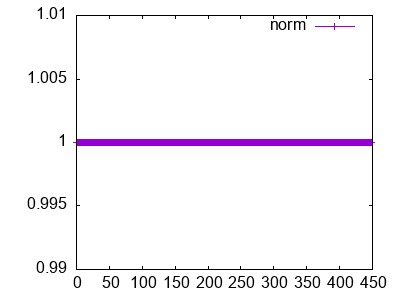
\includegraphics[width=0.6\textwidth]{norm.png}
    \caption[Squared Magnitude of the Wave Function over Time]{The
    \texttt{norm} axis indicates the sum of all the elements of
    $\vec{\Psi}(t)$.}
\end{figure}

The norm is one through all our time steps, so the implemented operator is
unitary, as we calculated. Now we examine the expected total energy,
momentum, and position for different $k$ values for a system with a constant
potential function and a potential well.

\pagebreak

\begin{center}
    \textit{Constant Potential}
\end{center}

We check to see if $\langle H \rangle \approx \frac{k^2}{2}$ and $\left|
\frac{d}{dt} \langle x \rangle \right| = \left| \langle p \rangle \right|
\approx k$, and that they behave roughly as explained in the
\nameref{sec:expected} section.

For $k = 0.59$, I computed with the programs
the following values.

\begin{figure}[H]
    \centering
    \begin{tabular}{cc}
        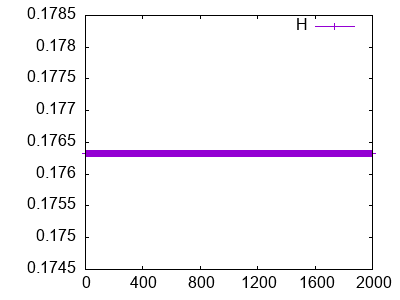
\includegraphics[width=0.4\textwidth]{Hc0.59.png}
        &
        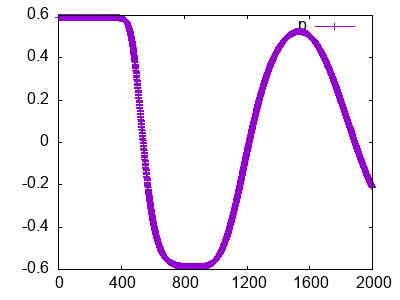
\includegraphics[width=0.4\textwidth]{pc0.59.png}
        \\
        (a) & (b)
        \\
        \multicolumn{2}{c}
        {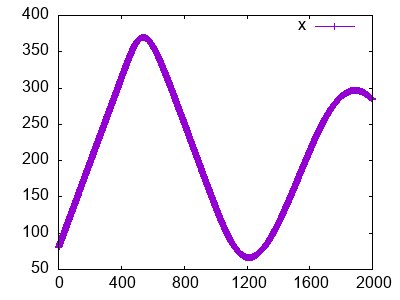
\includegraphics[width=0.4\textwidth]{xc0.59.png}}
        \\
        \multicolumn{2}{c}{(c)}
    \end{tabular}
    \caption[Expected Values over Time for $k = 0.59$]{The three plots
    display the expected values over time for $k = 0.59$. The $y$-axis in
    plot (a) indicates the total energy of the system. The $y$-axis in plots
    (b) and (c) indicate the expected momentum and expected position of the
    wave packet, respectively.}
    \label{fig:c0.59}
\end{figure}

The value $\frac{d}{dt} \langle x \rangle$ is equal to the slope in plot (c)
in Figure \ref{fig:c0.59}, which can be computed using the coorindates
$(x, t) = (0, 80), (81, 127.34)$ from the datafile: $\frac{d}{dt} \langle x
\rangle \approx 0.58 \approx k$. The computational expectation values for
the total energy of the system and momentum of the wave packet are
consistent with the theory.

\pagebreak

Now for $k = 1$, the programs output the following data.

\begin{figure}[H]
    \centering
    \begin{tabular}{cc}
        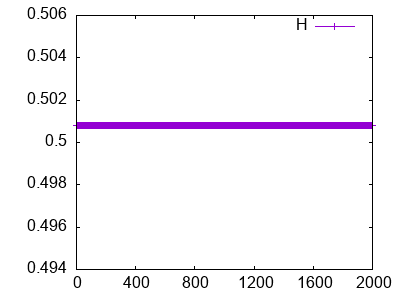
\includegraphics[width=0.4\textwidth]{Hc1.png}
        &
        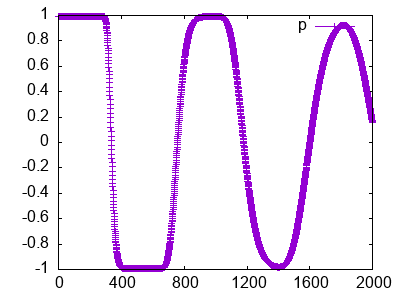
\includegraphics[width=0.4\textwidth]{pc1.png}
        \\
        (a) & (b)
        \\
        \multicolumn{2}{c}{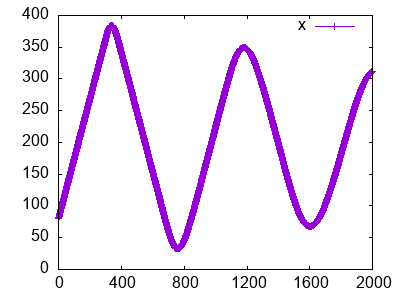
\includegraphics[width=0.4\textwidth]{xc1.png}}
        \\
        \multicolumn{2}{c}{(c)}
    \end{tabular}
    \caption[Expected Values over Time for $k = 1$]{The three plots display
    the expected values over time for $k = 1$. The $y$-axis in plot (a)
    indicates the total energy of the system. The $y$-axis in plots (b) and
    (c) indicate the expected momentum and expected position of the wave
    packet, respectively.}
    \label{fig:c1}
\end{figure}

The value $\frac{d}{dt} \langle x \rangle$ is equal to the slope in plot (c)
in Figure \ref{fig:c1}, which can be computed using the coorindates $(x, t)
= (0, 80), (81, 156.43)$ from the datafile: $\frac{d}{dt} \langle x \rangle
\approx 0.94 \approx k$. The wave packet moves over more distance in the
same amount of time for a larger $k$. The computational expectation values
are consistent with the theory.

\pagebreak

\begin{center}
    \textit{Finite Potential Square Well}
\end{center}

I used the following potential well.

\begin{figure}[H]
    \centering
    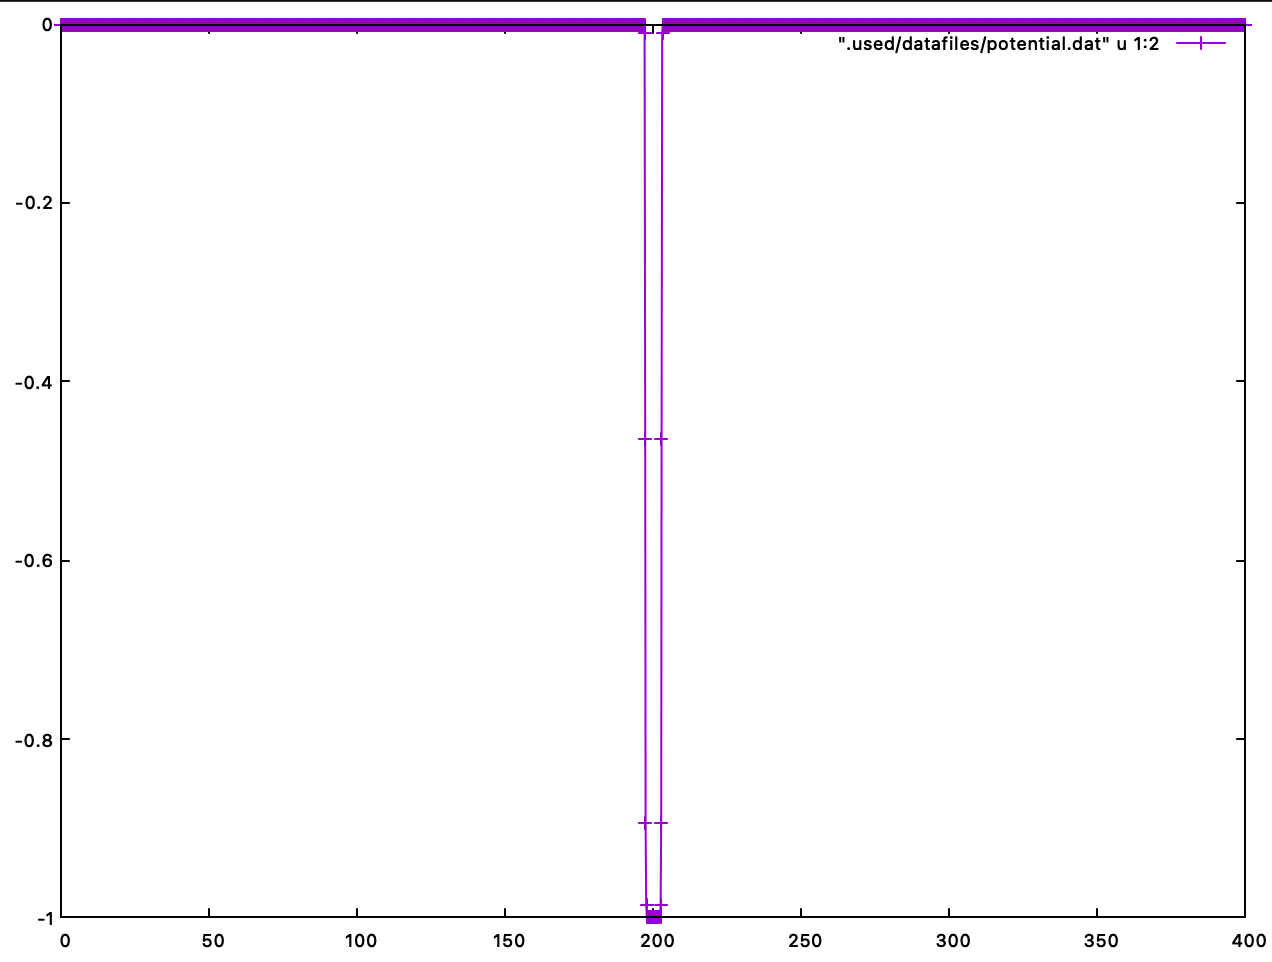
\includegraphics[width=0.6\textwidth]{smallwell.png}
    \caption[Small Potential Well]{The $y$-axis represents the potential
    energy, and the $x$-axis represents the position within the box.}
    \label{fig:smallwell}
\end{figure}

We check to see if $\langle H \rangle \approx \frac{k^2}{2}$ and if
initially $\left| \frac{d}{dt} \langle x \rangle \right| = \left| \langle p
\rangle \right| \approx k$, and that they behave roughly as explained in the
\nameref{sec:expected} section. The width of the well used was $0.01R$, and
the full width at half maximum (FWHM) of the Gaussian scalar function of the
initial wave packet used is $20\sqrt{2\log(2)}$ in $x$ space.

Figure \ref{fig:w} on the next page shows the numerical computations of the
expected value of each of the physical quantities for $k = 0.59, 1$, as
calculated by the programs.

\begin{figure}[H]
    \centering
    \begin{tabular}{ccc}
        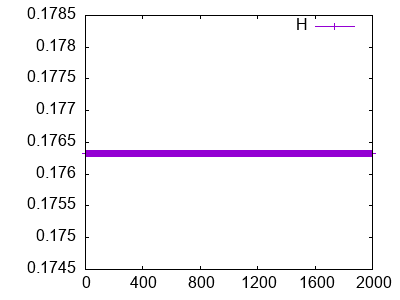
\includegraphics[width=0.3\textwidth]{Hw0.59.png}
        &
        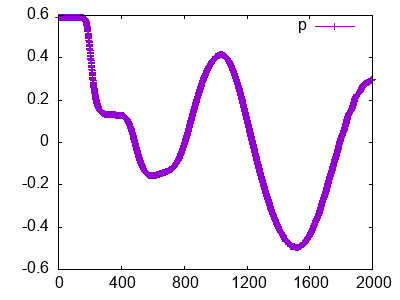
\includegraphics[width=0.3\textwidth]{pw0.59.png}
        &
        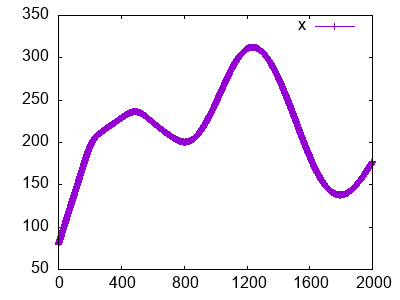
\includegraphics[width=0.3\textwidth]{xw0.59.png}
        \\
        (a) & (b) & (c)
        \\
        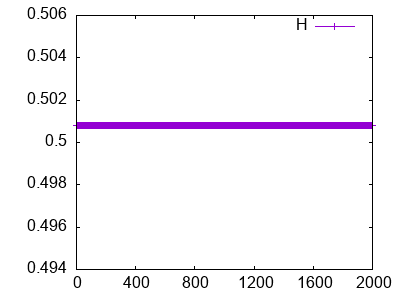
\includegraphics[width=0.3\textwidth]{Hw1.png}
        &
        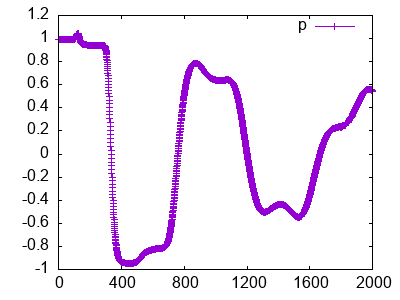
\includegraphics[width=0.3\textwidth]{pw1.png}
        &
        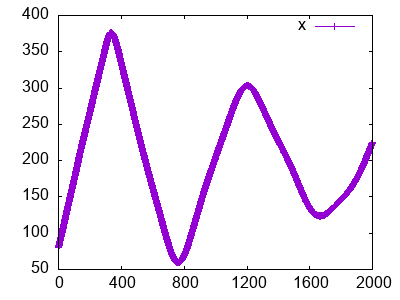
\includegraphics[width=0.3\textwidth]{xw1.png}
        \\
        (d) & (e) & (f)
    \end{tabular}
    \caption[Expected Values for a Large Well for $k = 0.59, 1$]{The top
    three plots display the expected values over time for
    $k = 0.59$, and the bottom three for $k = 1$. The $y$-axis in plots (a)
    and (d) indicates the total energy of the system. The $y$-axis in plots
    (b) and (e) indicates the expected momentum, and the $y$-axis in plots
    (c) and (f) indicates the expected position of the wave packet.}
    \label{fig:w}
\end{figure}

Although we will not compute the initial slope of plots (c) and (f), we may
notice that the predicted change in the expected position is represented in
the graphs, so the computational expected values are consistent with the
theory. The discrepancies between the graphs for $k = 0.59$ and $k = 1$ will
be discussed in further detail in the \nameref{subsec:num} subsection.

\addcontentsline{toc}{subsubsection}{Autocorrelation for $\left| \Psi
\right| ^ 2$ through Negative Time}
\subsubsection*{Autocorrelation for $\left| \Psi \right| ^ 2$ through
Negative Time}

We assess correctness with autocorrelation by checking if it is
approximately equal to one.  The following is the schema for measuring
autocorrelation, where $n \in \mathbb{Z}$.

\begin{align*}
    \Psi(n \delta t) &=
    \left(
    \frac{1 - iH\frac{\delta t}{2}}{1 + iH\frac{\delta t}{2}}
    \right)^n
    \Psi(0)
    \\
    {\tilde{\Psi}}_n(0) &=
    \left(
    \frac{1 - iH\frac{-\delta t}{2}}{1 + iH\frac{-\delta t}{2}}
    \right)^n
    \Psi(n \delta t)
    \\
    \mathrm{autocorrelation} &=
    \int_0^R \Psi(0)^* \tilde{\Psi}(0) dx
\end{align*}

To implement this measure using the implicit scheme of propagation, I
propagated forward in time by $n$ time steps, and backward in time by the
same number of time steps. The integral was calculated by summing the
product of each element of $\vec{\Psi}(0)$ and the complex conjugate of its
corresponding element of $\vec{\tilde{\Psi}}(0)$.

\begin{figure}[H]
    \centering
    
\includegraphics[width=0.7\textwidth]{autocorr.out.png}
    \caption[Autocorrelation output]{The output for the autocorrelation for
    $\delta t = 0.9$ and the $n = 2222$.}
\end{figure}

The autocorrelation is exactly equal to one because the error in forward
propagation is equal to the negative of the backward negative operator
because a factor of the propagator error, $\delta t^3$, is odd with respect
to $\delta t$.

\addcontentsline{toc}{subsection}{Numerical Calculations of the Transmission
Coefficient}
\subsection*{Numerical Calculations of the Transmission Coefficient}
\label{subsec:num}

I numerically calculated the transmission coefficient by

\[
    \sum_{j = A}^N \vec{\Psi}_j(t_f)
\]

where $A$ is the number of spacial steps that corresponds to the approximate
edge of the well that is on the side opposite of the starting position of
the wave packet, $N$ is again the total number of spacial steps. This
summation is computed at $t_f$, corresponding to a time after the full
transmission through the well has occured.

\begin{figure}[H]
    \centering
    \begin{tabular}{cc}
        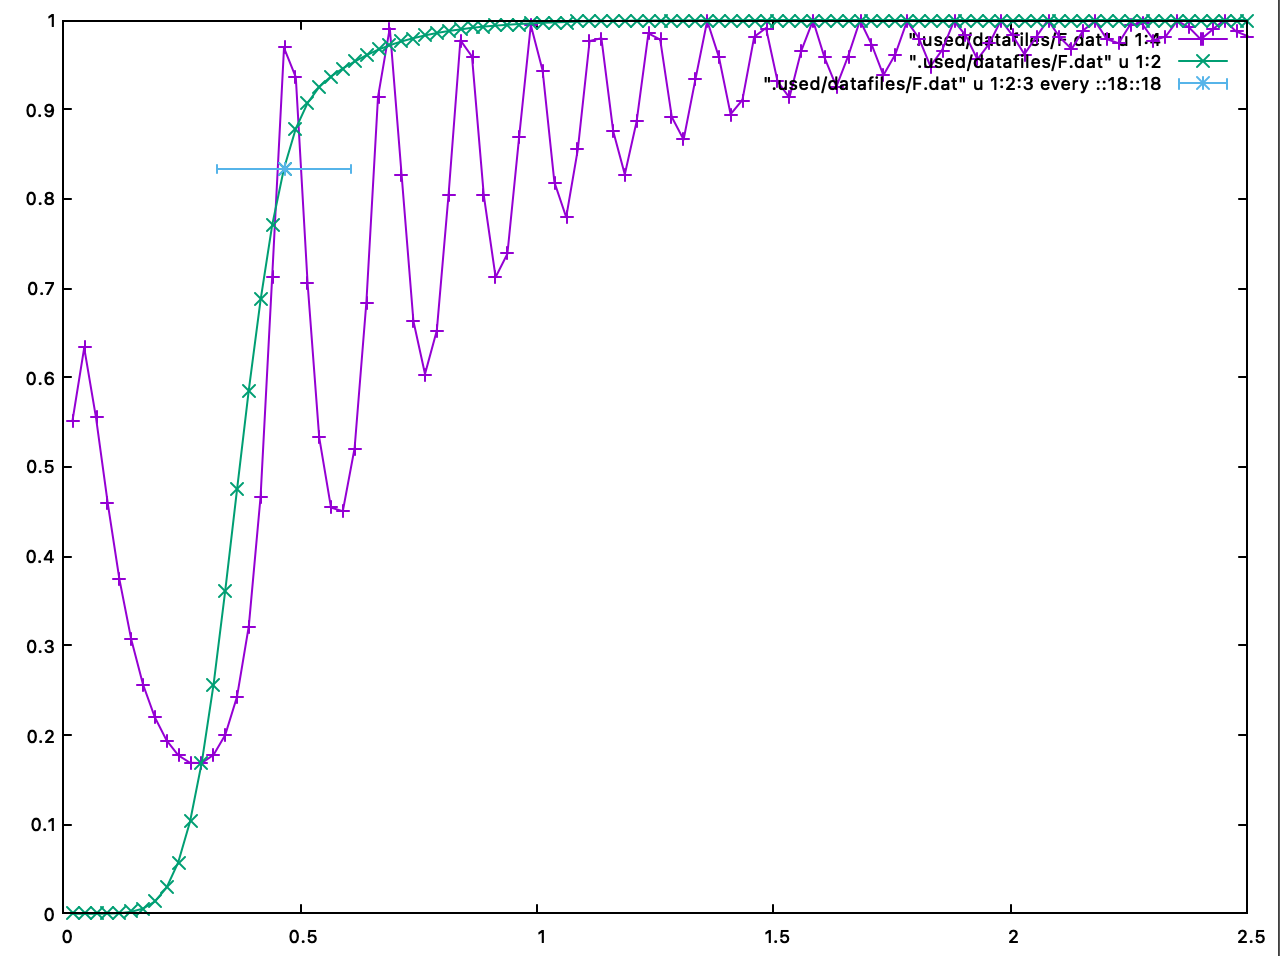
\includegraphics[width=0.4\textwidth]{translarge.png}
        &
        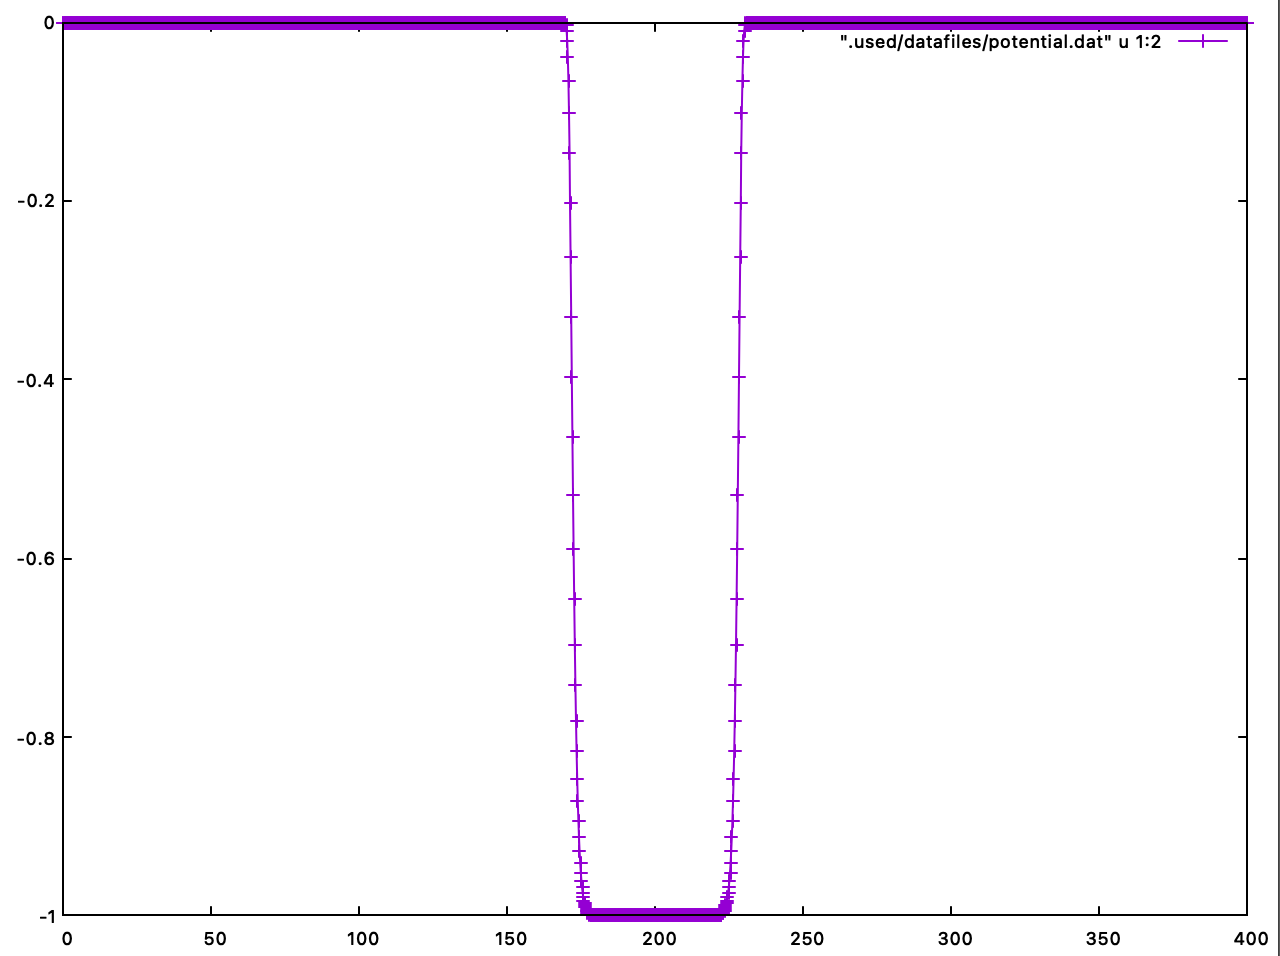
\includegraphics[width=0.4\textwidth]{largewell.png}
        \\
        (a) & (b)
    \end{tabular}
    \caption[Large Well Transmission]{The $x$-axis represents $k$. The
    transmission coefficient as calculated analytically is plotted in purple
    and as computed numerically is plotted in turquoise. The length of each
    side of the error bar is the half width of the wave packet in $k$ space,
    calculated by $\frac{2}{\sqrt{2\sigma^2}}$ where $\sigma$ is the
    standard deviation parameter for the Gaussian envelope.}
    \label{translarge}
\end{figure}

We see that the numerical computation does not match the analytical solution.
If we recall that the analytical solution is for an eigenstate, and that a
wave packet is superposition of many eigenstates, it is then reasonable to
guess that the plot of the numerical solution appears as sort of an
$S$-curve because the transmission of all plane waves composing the wave
packet, each of which corresponds to its own $k$ value, are summed, and that
the center of the $k$ distribution is larger than one oscillation in the
analytical solution. We must reduce the width of the wave packet in
$k$-space in order for the numerical plot to resemble the analytical plot.
This corresponds to a decrease in the width of the wave packet in $x$-space,
which at this point we may reduce the width of the well to maintain an
approximately infinitely large box\footnote[1]{The relation between the well
width in $x$-space and $k$-space is calculated by Fourier transform and
FWHM of the wave packet.}. The graph (a) in Figure \ref{translarge} uses a
well width of $0.1R$, seen in graph (b). The following figure uses a well
width of $0.01R$, seen in Figure \ref{fig:smallwell}.

\begin{figure}[H]
    \centering
    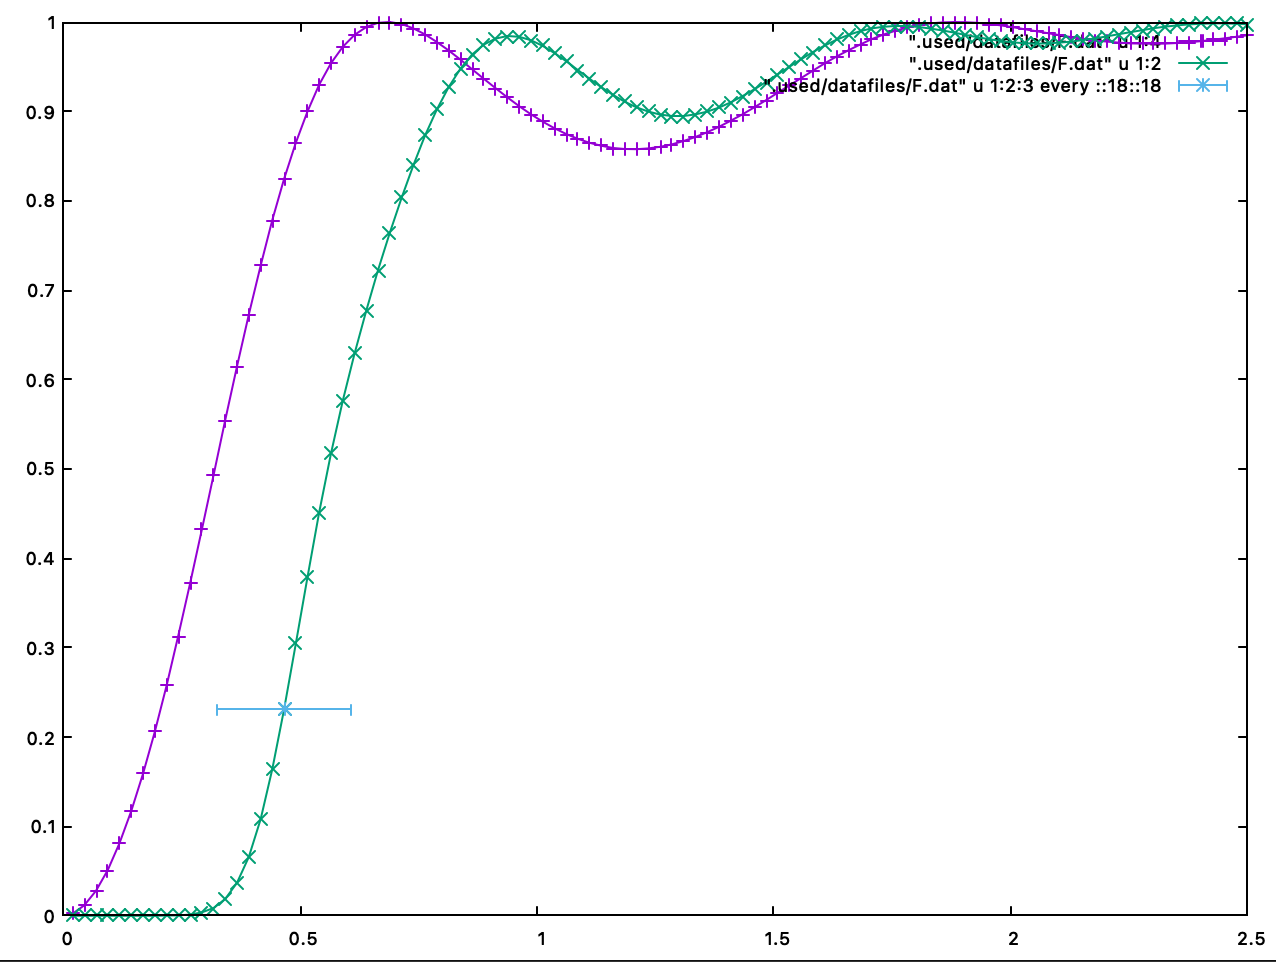
\includegraphics[width=0.6\textwidth]{transsmall.png}
    \caption[Small Well Transmission]{The plots are the same as in Figure
    \ref{translarge}.}
\end{figure}

We see now that the error bar is smaller than one oscillation in the
analytical plot, and that both functions match with an offset of some phase
constant.

Revisiting the graphs for the expected values over time for a system with a
finite potential well (Figure \ref{fig:w}), we noted the differences in the
expected values over $k = 0.59$ and $k = 1$. If we compare those to the
graphs in Figures \ref{fig:c0.59} and \ref{fig:c1}, we see that the expected
values behave more similarly between a constant potential and a potential
well for $k = 1$ than $k = 0.59$. This is because there is a larger
transmission at $k = 0.59$, which is supported by the analytical plot.

\addcontentsline{toc}{subsubsection}{Extended Verification}
\subsubsection*{Extended Verification}

We extend our verification process by examining the wave packet and
transmission over time over $k$. We notice a reflection and transmission in
Figure \ref{fig:wellanim}, and an oscillation in transmission (equal to the
plateau since the initial wave packet is normalized) through $k$ in Figure
\ref{fig:Fanim}.

\begin{figure}[H]
    \centering
    \begin{tabular}{cc}
        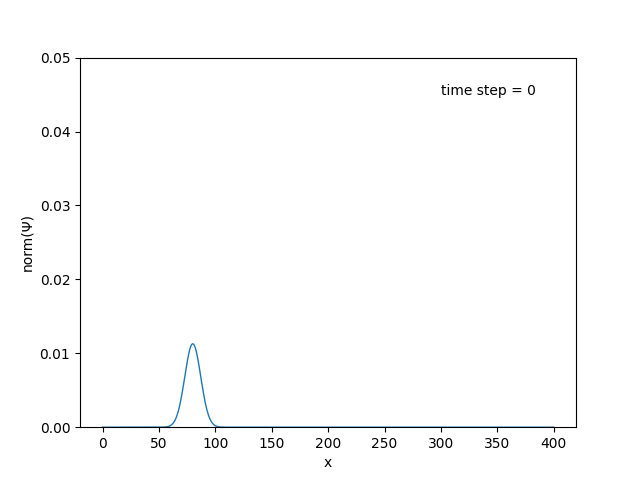
\includegraphics[width=0.4\textwidth]{well1.png}
        &
        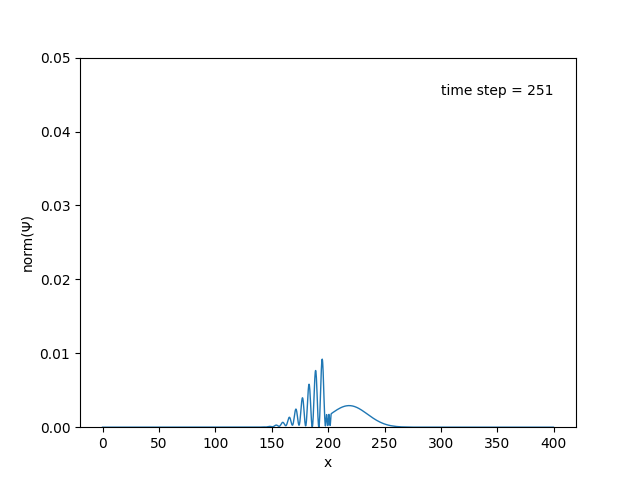
\includegraphics[width=0.4\textwidth]{well252.png}
        \\
        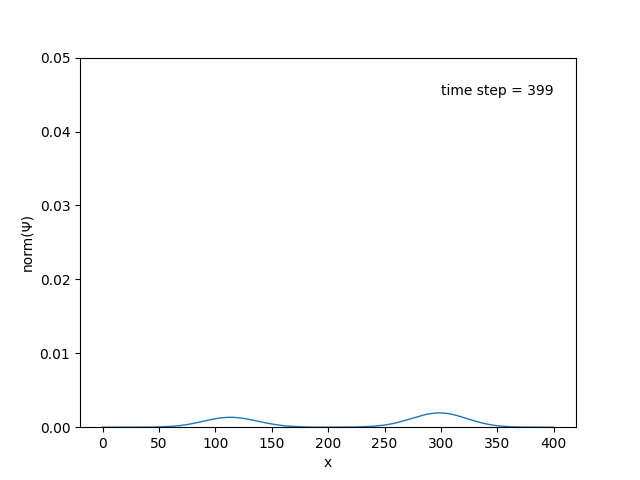
\includegraphics[width=0.4\textwidth]{well400.png}
        &
        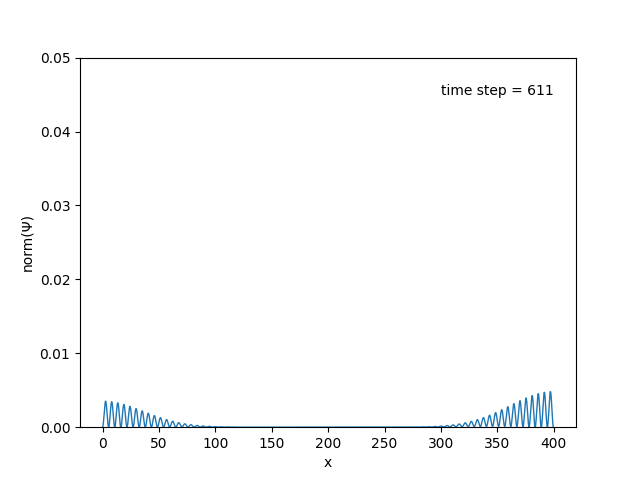
\includegraphics[width=0.4\textwidth]{well612.png}
    \end{tabular}
    \caption[Well Propagation]{The square magnitude of the wave packet at
    four different time steps}
    \label{fig:wellanim}
\end{figure}

\begin{figure}[H]
    \centering
    \begin{tabular}{ccc}
        \includegraphics[width=0.3\textwidth]{F10.png}
        &
        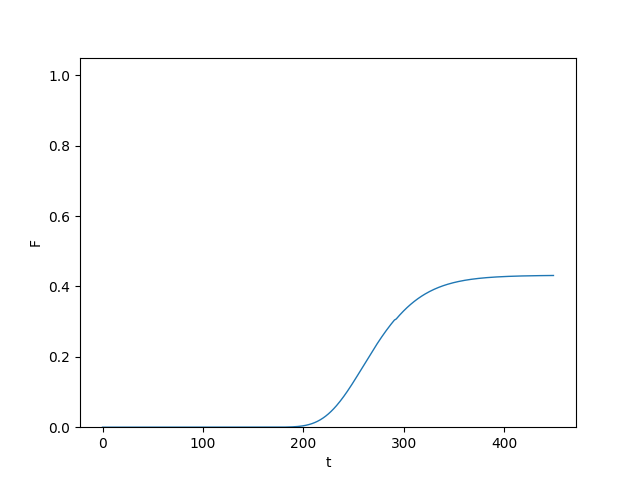
\includegraphics[width=0.3\textwidth]{F20.png}
        &
        \includegraphics[width=0.3\textwidth]{F46.png}
    \end{tabular}
    \begin{tabular}{cc}
        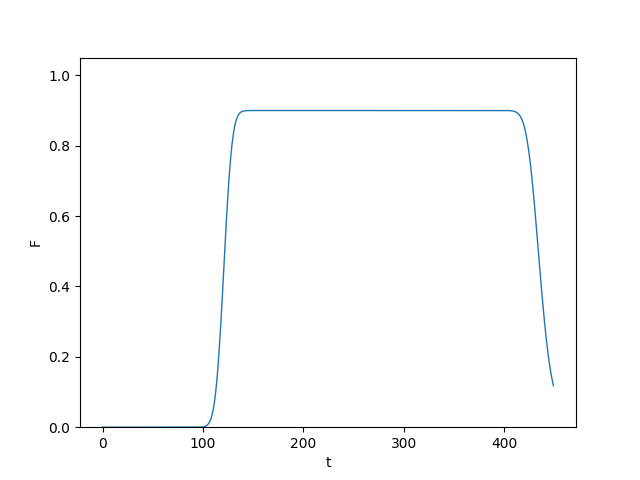
\includegraphics[width=0.3\textwidth]{F55.png}
        &
        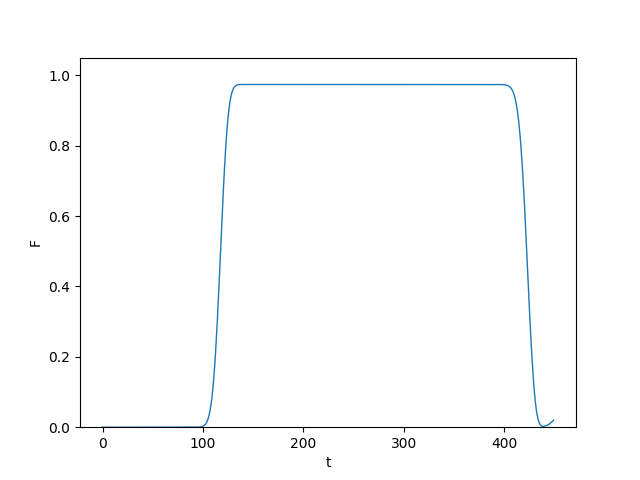
\includegraphics[width=0.3\textwidth]{F65.png}
    \end{tabular}
    \caption[Transmission Probabilities]{The probability of the localized
    particle being transmitted ($F$) over time for increasing $k$}
    \label{fig:Fanim}
\end{figure}


\end{document}
